\documentclass[class=article,10pt,crop=false]{standalone}
\usepackage{standalone}
\usepackage{preamble}

%Break line: In Neville's algorithm (interpolation section-polynomial interpolation)
\begin{document}
\begin{multicols}{2}[\section{Numerical methods}]
\subsection{Errors}
\subsubsection*{Floating-point representation}
\begin{theorem}
Let $b\in\mathbb{N}$, $b\geq 2$. Any real number $x\in\mathbb{R}$ can be represented of the form 
\begin{equation*}
    x=s\left(\sum_{i=1}^\infty\alpha_ib^{-i}\right)b^q,
\end{equation*} where $s\in\{-1,1\}$, $q\in\mathbb{Z}$ and $\alpha_i\in\{0,1,\ldots,b-1\}$. Moreover, this representation is unique if $\alpha_1\ne0$ and $\forall i_0\in\mathbb{N}$, $\exists i\geq i_0:\alpha_i\ne b-1$. We will write $$x=s(0.\alpha_1\alpha_2\cdots)_bb^q,$$ where the subscript $b$ in the parenthesis indicates that the number $0.\alpha_1\alpha_2\alpha_3\cdots$ is in base $b$.
\end{theorem}
\begin{definition}[Floating-point representation]
Let $x$ be a real number. Then the floating-point representation of $x$ is $$x=s\left(\sum_{i=1}^t\alpha_ib^{-i}\right)b^q.$$ Here $s$ is called the \textit{sign}; $\sum_{i=1}^t\alpha_ib^{-i}$, the \textit{significant} or \textit{mantissa}, and $q$, the \textit{exponent}, limited to a prefixed range $q_\text{min}\leq q\leq q_\text{max}$. So, the floating-point representation of $x$ is $$x=smb^q=s(0.\alpha_1\alpha_2\cdots\alpha_t)_bb^q.$$ Finally we say a floating-point number is \textit{normalized} if $\alpha_1\ne0$.
\end{definition}
\begin{table}[ht]
    \centering
    \begin{tabular}{c|ccccc}
        Format & $b$ & $t$ & $q_\text{min}$ & $q_\text{max}$ & bits \\
        \hline\hline
        IEEE simple & 2 & 24 & -126 & 127 & 32\\
        IEEE double & 2 & 53 & -1022 & 1023 & 64
    \end{tabular}
    \caption{Parameters of IEEE simple and IEEE double formats.}
    \label{tab:my_label}
\end{table}
\begin{definition}
We define $F(b,t,q_\text{min},q_\text{max})$ as:
\begin{multline*}
    F(b,t,q_\text{min},q_\text{max}):=\{0\}\cup\{\pm(0.\alpha_1\alpha_2\cdots\alpha_t)_bb^q:\\\alpha_i\in\{0,1,\ldots,b-1\},\alpha_1\ne0, q_\text{min}\leq q\leq q_\text{max}\}.
\end{multline*}
\end{definition}
\begin{definition}
Let $x\in\mathbb{R}$ be such that $x=s(0.\alpha_1\alpha_2\cdots)_bb^q$ with $q_\text{min}\leq q\leq q_\text{max}$. We say the \textit{floating-point representation by truncation of $x$} is $$fl_T(x)=s(0.\alpha_1\alpha_2\cdots\alpha_t)_bb^q.$$ We say the \textit{floating-point representation by rounding of $x$} is
\begin{multline*}
fl_R(x)=\\=\left\{\text{\setlength{\tabcolsep}{4pt}\begin{tabular}{m{3.85cm}m{3cm}}
        $s(0.\alpha_1\cdots\alpha_t)_bb^q$ & if $\ 0\leq\alpha_{t+1}<\frac{b}{2}$\\
        $s(0.\alpha_1\cdots\alpha_{t-1}(\alpha_t+1))_bb^q$ & if $\ \frac{b}{2}\leq\alpha_{t+1}\leq b-1.$
    \end{tabular}}\right.
\end{multline*}
\end{definition}
\begin{definition}
Given a value $x\in\mathbb{R}$ and an approximation $\Tilde{x}$ of $x$, the \textit{absolute error} is $$\Delta x:=|x-\Tilde{x}|.$$ If $x\ne 0$, the \textit{relative error} is $$\delta x:=\frac{|x-\Tilde{x}|}{x}.$$ If $x$ is unknown, we will take $$\delta x\approx\frac{|x-\Tilde{x}|}{\Tilde{x}}.$$
\end{definition}
\begin{definition}
Let $\Tilde{x}$ be an approximation of $x$. If $\Delta x\leq\frac{1}{2}10^{-t}$, we say \textit{$\Tilde{x}$ has $t$ correct decimal digits}. If $x=sm10^q$ with $0.1\leq m<1$, $\Tilde{x}=s\Tilde{m}10^q$ and $$u:=\max\{i\in\mathbb{Z}:|m-\Tilde{m}|\leq\frac{1}{2}10^{-i}\},$$ then we say that $\Tilde{x}$ \textit{has $u$ significant digits}.
\end{definition}
\begin{prop}
Let $x\in\mathbb{R}$ be such that $x=s(0.\alpha_1\alpha_2\cdots)_bb^q$ with $\alpha_1\ne0$ and $q_\text{min}\leq q\leq q_\text{max}$. Then, we have:
\begin{align*}
    \left|fl_T(x)-x\right|\leq b^{q-t},\quad&\quad \left|fl_R(x)-x\right|\leq\frac{1}{2}b^{q-t}.\\
    \left|\frac{fl_T(x)-x}{x}\right|\leq b^{1-t},\quad&\quad \left|\frac{fl_R(x)-x}{x}\right|\leq\frac{1}{2}b^{1-t}.
\end{align*}
\end{prop}
\begin{definition}
The \textit{machine epsilon $\epsilon$} is defined as $$\epsilon:=\min\{\varepsilon>0:fl(1+\varepsilon)\ne 1\}.$$
\end{definition}
\begin{prop}
For a machine working by truncation, $\epsilon=b^{1-t}$. For a machine working by rounding, $\epsilon=\frac{1}{2}b^{1-t}$.
\end{prop}
\subsubsection*{Propagation of errors}
\begin{prop}[Propagation of absolute errors]
Let $f:\mathbb{R}^n\rightarrow\mathbb{R}$ be a function of class $\mathcal{C}^2$. If $\Delta x_j$ is the absolute error of the variable $x_j$ and $\Delta f(x)$ is the absolute error of the function $f$ evaluated at the point $x=(x_1,\ldots,x_n)$, we have $$|\Delta f(x)|\lesssim\sum_{j=1}^n\left|\frac{\partial f}{\partial x_j}(x)\right||\Delta x_j|\footnote{The symbol $\lesssim$ means that we are omitting terms of order $\Delta x_j\Delta x_k$ and higher.}.$$ The coefficients $\displaystyle\frac{\partial f}{\partial x_j}(x)$ are called \textit{absolute condition numbers of the problem}. 
\end{prop}
\begin{prop}[Propagation of relative errors]
Let $f:\mathbb{R}^n\rightarrow\mathbb{R}$ be a function of class $\mathcal{C}^2$. If $\delta x_j$ is the relative error of the variable $x_j$ and $\delta f(x)$ is the relative error of the function $f$ evaluated at the point $x=(x_1,\ldots,x_n)$, we have $$|\delta f(x)|\lesssim\sum_{j=1}^n\frac{\left|\frac{\partial f}{\partial x_j}(x)\right|\left|x_j\right|}{\left|f(x)\right|}|\delta x_j|.$$ The coefficients $\displaystyle \left|\frac{\partial f}{\partial x_j}(x)\right|\left|x_j\right|/\left|f(x)\right|$ are called \textit{relative condition numbers of the problem}. 
\end{prop}
\subsubsection*{Numerical stability of algorithms}
\begin{definition}
An algorithm is said to be \textit{numerically stable} if  errors in the input lessen in significance as the algorithm executes, having little effect on the final output. On the other hand, an algorithm is said to be \textit{numerically unstable} if errors in the input cause a considerably larger error in the final output.
\end{definition}
\begin{definition}
A problem with a low condition number is said to be \textit{well-conditioned}. Conversely, a problem with a high condition number is said to be \textit{ill-conditioned}.
\end{definition}
\subsection{Zeros of functions}
\begin{definition}
Let $f:\mathbb{R}\rightarrow\mathbb{R}$ be a function. We say $\alpha$ is a \textit{zero} or a \textit{solution to the equation $f(x)=0$} if $f(\alpha)=0$.
\end{definition}
\begin{definition}
Let $f:\mathbb{R}\rightarrow\mathbb{R}$ be a function. We say $\alpha$ is a \textit{zero of multiplicity $m$} if $$f(\alpha)=f'(\alpha)=\cdots=f^{(m-1)}(\alpha)=0\quad\text{and}\quad f^{(m)}\ne0.$$ If $m=1$, the zero is called \textit{simple}; if $m=2$, \textit{double}...
\end{definition}
\subsubsection*{Root-finding methods}
For the following methods consider a continuous function $f:I\subseteq\mathbb{R}\rightarrow\mathbb{R}$ with an unknown zero $\alpha\in I$. Given a $\varepsilon>0$, we want to approximate the value of $\alpha$ with $\Tilde{\alpha}$, such that $|\alpha-\Tilde{\alpha}|<\varepsilon$.
\begin{theorem}[Bisection method]
Suppose $I=[a_0,b_0]$. For each step $n\geq 0$ of the algorithm we will approximate $\alpha$ by $$c_n=\frac{a_n+b_n}{2}.$$ If $f(c_n)=0$ we are done. If not, let
$$[a_{n+1},b_{n+1}]=\left\{\begin{array}{ccc}
    [a_n,c_n] & \text{if} & f(a_n)f(c_n)<0, \\
    \left[c_n,b_n\right] & \text{if} & f(a_n)f(c_n)>0.
\end{array}\right.$$ and iterate the process again. Observe the length of the interval $[a_n,b_n]$ is $\frac{b_0-a_0}{2^n}$. Note that: $$|\alpha-c_n|<\frac{b_0-a_0}{2^{n+1}}<\varepsilon\iff n>\frac{\log\left(\frac{b_0-a_0}{\varepsilon}\right)}{\log 2}-1.$$
\end{theorem}
\begin{theorem}[\textit{Regula falsi} method]
Suppose $I=[a_0,b_0]$. For each step $n\geq 0$ of the algorithm we will approximate $\alpha$ by $$c_n=b_k-f(b_k)\frac{b_k-a_k}{f(b_k)-f(a_k)}=\frac{a_kf(b_k)-b_kf(a_k)}{f(b_k)-f(a_k)}.$$ If $f(c_n)=0$ we are done. If not, let
$$[a_{n+1},b_{n+1}]=\left\{\begin{array}{ccc}
    [a_n,c_n] & \text{if} & f(a_n)f(c_n)<0, \\
    \left[c_n,b_n\right] & \text{if} & f(a_n)f(c_n)>0,
\end{array}\right.$$ and iterate the process again.
\end{theorem}
\begin{theorem}[Secant method]
Suppose $I=\mathbb{R}$ and that we have two different initial approximations $x_0$, $x_1$. Then for each step $n\geq 0$ of the algorithm we obtain a new approximation $x_{n+2}$, given by: $$x_{n+2}=\frac{x_nf(x_{n+1})-x_{n+1}f(x_n)}{f(x_{n+1})-f(x_n)}.$$
\end{theorem}
\begin{theorem}[Newton–Raphson method]
Suppose $I=\mathbb{R}$, $f\in\mathcal{C}^1$ and that we have an initial approximation $x_0$. Then for each step $n\geq 0$ we obtain a new approximation $x_{n+1}$, given by: $$x_{n+1}=x_n-\frac{f(x_n)}{f'(x_n)}.$$
\end{theorem}
\begin{theorem}[Chebyshev method]
Suppose $I=\mathbb{R}$, $f\in\mathcal{C}^2$ and that we have an initial approximation $x_0$. Then for each step $n\geq 0$ we obtain a new approximation $x_{n+1}$, given by: $$x_{n+1}=x_n-\frac{f(x_n)}{f'(x_n)}-\frac{1}{2}\frac{\left[f(x_n)\right]^2f''(x_n)}{\left[f'(x_n)\right]^3}.$$
\end{theorem}
\subsubsection*{Fixed point methods}
\begin{definition}
Let $g:[a,b]\rightarrow[a,b]\subset\mathbb{R}$ be a function. A point $\alpha\in[a,b]$ is \textit{n-periodic} if $g^n(\alpha)=\alpha$ and $g^j(\alpha)\ne\alpha$ for $j=1,\ldots,n-1$\footnote{Note that 1-periodic points are the fixed points of $f$.}.
\end{definition}
\begin{theorem}[Fixed point theorem]
Let $(M,d)$ be a metric space and $g:M\rightarrow M$ a contraction\footnote{Remember definitions \ref{FOSV_metric} and \ref{FOSV_contr}.}. Then $g$ has a unique fixed point $\alpha\in M$ and for every $x_0\in E$, $$\alpha=\lim_{n\to\infty}x_n,\quad\text{where }x_n=g(x_{n-1})\quad\forall n\in\mathbb{N}.$$
\end{theorem}
\begin{prop}
Let $(M,d)$ be a metric space and $g:M\rightarrow M$ a contraction of constant $k$. Then if we want to approximate a fixed point $\alpha$ by the iteration $x_n=g(x_{n-1})$, we have:
\begin{align*}
    d(x_n,\alpha)&\leq\frac{k^n}{1-k}d(x_1,x_0)\quad&\text{(a priori estimation)}\\
    d(x_n,\alpha)&\leq\frac{k}{1-k}d(x_n,x_{n-1})\quad&\text{(a posteriori estimation)}
\end{align*}
\end{prop}
\begin{corollary}
Let $g:\mathbb{R}\rightarrow\mathbb{R}$ be a function of class $\mathcal{C}^1$. Suppose $\alpha$ is a fixed point of $g$ and $|g'(\alpha)|<1$. Then, there exists $\varepsilon>0$ such that $g$ is a contraction on $[\alpha-\varepsilon,\alpha+\varepsilon]$. In particular, the iteration $x_{n+1}=g(x_n)$ converges to $\alpha$.
\end{corollary}
\begin{definition}
Let $g:\mathbb{R}\rightarrow\mathbb{R}$ be a function of class $\mathcal{C}^1$ and $\alpha$ be a fixed point of $g$. We say $\alpha$ is an \textit{attractor fixed point} if $|g'(\alpha)|<1$. In this case, any iteration $x_{n+1}=g(x_n)$ converges to $\alpha$. If $|g'(\alpha)|>1$, we say $\alpha$ is a \textit{repulsor fixed point}. In this case, any iteration $x_{n+1}=g(x_n)$ doesn't converge to $\alpha$.
\end{definition}
\begin{minipage}{\linewidth}
    \centering
    \begin{minipage}{0.49\linewidth} 
        \centering
        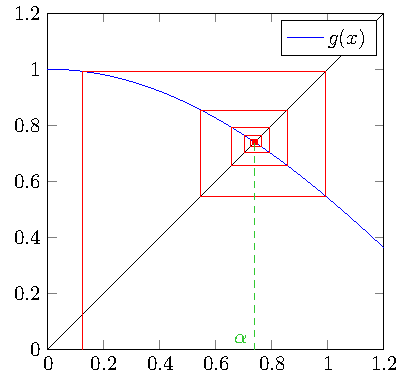
\includegraphics[width=\linewidth]{Mathematics/2nd/Numerical_methods/Images/cobweb1.tex} 
    \end{minipage}\hfill
    \begin{minipage}{0.49\linewidth} 
        \centering
        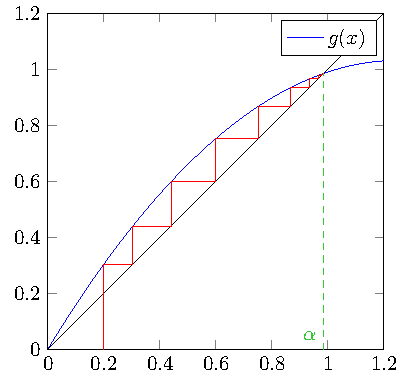
\includegraphics[width=\linewidth]{Mathematics/2nd/Numerical_methods/Images/cobweb2.tex} 
    \end{minipage}
    \captionof{figure}{Cobweb diagrams}
\end{minipage}
\subsubsection*{Order of convergence}
\begin{definition}[Order of convergence]
Let $(x_n)$ be a sequence of real numbers that converges to $\alpha\in\mathbb{R}$. We say $(x_n)$ has \textit{order of convergence $p\in\mathbb{R}^+$} if exists $C>0$ such that: $$\lim_{n\to\infty}\frac{|x_{n+1}-\alpha|}{|x_n-\alpha|^p}=C.$$ The constant $C$ is called \textit{asymptotic error constant}. For the case $p=1$, we need $C<1$. In this case the convergence is called \textit{linear convergence}; for $p=2$, is called \textit{quadratic convergence}; for $p=3$, \textit{cubic convergence}... If it's satisfied that $$\lim_{n\to\infty}\frac{|x_{n+1}-\alpha|}{|x_n-\alpha|^p}=0$$ for some $p\in\mathbb{R}$, we say the sequence has \textit{order of convergence at least $p$}.
\end{definition}
\begin{theorem}
Let $g:\mathbb{R}\rightarrow\mathbb{R}$ be a function of class $\mathcal{C}^p$ and let $\alpha$ be a fixed point of $g$. Suppose $$g'(\alpha)=g''(\alpha)=\cdots=g^{(p-1)}(\alpha)=0$$ with $|g'(\alpha)|<1$ if $p=1$. Then the iteration $x_{n+1}=g(x_n)$ has order of convergence at least $p$. If, moreover, $g^{(p)}(\alpha)\ne0$, then the previous iteration has order of convergence $p$ with asymptotic error constant $C=\frac{|g^{(p)}(\alpha)|}{p!}$.
\end{theorem}
\begin{theorem}
Let $f:\mathbb{R}\rightarrow\mathbb{R}$ be a function of class $\mathcal{C}^2$ and let $\alpha$ be a simple zero of $f$. If $f''(\alpha)\ne0$, then Newton's method for finding $\alpha$ has quadratic convergence with asymptotic error constant $C=\frac{1}{2}\left|\frac{f''(\alpha)}{f'(\alpha)}\right|$.\par If $f\in\mathcal{C}^{m+2}$, and $\alpha$ is a zero of multiplicity $m>1$, then Newton's method has a linear convergence.
\end{theorem}
\begin{theorem}
Let $f:\mathbb{R}\rightarrow\mathbb{R}$ be a function of class $\mathcal{C}^3$ and let $\alpha$ be a simple zero of $f$. Then Chebyshev's method for finding $\alpha$ has at least cubic convergence.
\end{theorem}
\begin{definition}
We define the \textit{computational efficiency of an algorithm} as a function $E(p,t)$, where $t$ is the time taken for each iteration of the method and $p$ is the order of convergence of the method. $E(p,t)$ must satisfy the following properties:
\begin{enumerate}
    \item $E(p,t)$ is increasing with respect to the variable $p$ and decreasing with respect to $t$.
    \item $E(p,t)=E(mt,p^m)$ $\forall m\in\mathbb{R}$.
\end{enumerate}
Examples of such functions are the following: $$E(p,t)=\frac{\log p}{t},\quad E(p,t)=p^{1/t}.$$
\end{definition}
\subsubsection*{Sequence acceleration}
\begin{definition}[Aitken's $\Delta^2$ method]
Let $(x_n)$ be a sequence of real numbers. We denote:
\begin{gather*}
    \Delta x_n:=x_{n+1}-x_n,\\\Delta^2 x_n:=\Delta x_{n+1}-\Delta x_n=x_{n+2}-2x_{n+1}+x_n.
\end{gather*}
\textit{Aitken's $\Delta^2$ method} is the transformation of the sequence $(x_n)$ into a sequence $y_n$, defined as: $$y_n:=x_n-\frac{(\Delta x_n)^2}{\Delta^2 x_n}=x_n-\frac{(x_{n+1}-x_n)^2}{x_{n+2}-2x_{n+1}+x_n}.$$
\end{definition}
\begin{theorem}
Let $(x_n)$ be a sequence of real numbers such that $\displaystyle\lim_{n\to\infty}x_n=\alpha$, $x_n\ne\alpha$ for all $n\in\mathbb{N}$ and $\exists C$, $|C|<1$, satisfying $$x_{n+1}-\alpha=(C+\delta_n)(x_n-\alpha),\quad\text{with }\lim_{n\to\infty}\delta_n=0.$$ Then the sequence $(y_n)$ obtained from Aitken's $\Delta^2$ process is well-defined and $$\lim_{n\to\infty}\frac{y_n-\alpha}{x_n-\alpha}=0\footnote{This means that Aitken's $\Delta^2$ method produces an acceleration of the convergence of the sequence $(x_n)$.}.$$
\end{theorem}
\begin{theorem}[Steffensen's method]
Let $g:\mathbb{R}\rightarrow\mathbb{R}$ be a continuous function and suppose we have an iterative method $x_{n+1}=g(x_n)$. Then for each step $n$ we can consider a new iteration $y_{n+1}$, given by: \begin{multline*}
    y_{n+1}=y_n-\frac{\left[g(y_n)-y_n\right]^2}{g(g(y_n))-2g(y_n)+y_n}=\\=\frac{y_ng(g(y_n))-\left[g(y_n)\right]^2}{g(g(y_n))-2g(y_n)+y_n}.
\end{multline*}
\end{theorem}
\begin{prop}
Let $f:\mathbb{R}\rightarrow\mathbb{R}$ be a function of class $\mathcal{C}^2$ and let $\alpha$ be a simple zero of $f$. Then Steffensen's method for finding $\alpha$ has at least quadratic convergence\footnote{Note that the advantage of Steffensen's method over Newton's method is that in the former we don't need the differentiability of the function whereas in the latter we do.}.
\end{prop}
\subsubsection*{Zeros of polynomials}
\begin{lemma}
Let $p(z)=a_0+a_1z+\cdots+a_nz^n\in\mathbb{C}[x]$ with $a_n\ne 0$. We define $$\lambda:=\max\left\{\left|\frac{a_i}{a_n}\right|:i=0,1,\ldots,n-1\right\}.$$ Then if $p(\alpha)=0$ for some $\alpha\in\mathbb{C}$, $\|\alpha\|\leq\lambda+1$.
\end{lemma}
\begin{definition}[Strum's sequence]
Let $(f_i)$, $i=0,\ldots,n$, be a sequence of continuous functions defined on $[a,b]\subset\mathbb{R}$ and $f:[a,b]\rightarrow\mathbb{R}$ be a function of class $\mathcal{C}^1$ such that $f(a)f(b)\ne 0$. We say $(f_n)$ is a \textit{Sturm's sequence} if:
\begin{enumerate}
    \item $f_0=f$.
    \item If $\alpha\in[a,b]$ satisfies $f_0(\alpha)=0\implies f_0'(\alpha)f_1(\alpha)>0$.
    \item For $i=1,\ldots,n-1$, if $\alpha\in[a,b]$ satisfies $f_i(\alpha)=0\implies f_{i-1}(\alpha)f_{i+1}(\alpha)<0$.
    \item $f_n(x)\ne0$ $\forall x\in[a,b]$.
\end{enumerate}
\end{definition}
\begin{definition}
Let $(a_i)$, $i=0,\ldots,n$, be a sequence. We define $\nu(a_i)$ as the number of sign variations of the sequence $$\{a_0,a_1,\ldots,a_n\},$$ without taking into account null values. 
\end{definition}
\begin{theorem}[Sturm's theorem]
Let $f:[a,b]\rightarrow\mathbb{R}$ be a function of class $\mathcal{C}^1$ such that $f(a)f(b)\ne 0$ and with a finite number of zeros. Let $(f_i)$, $i=0,\ldots,n$, be a Sturm sequence defined on $[a,b]$. Then the number of zeros of $f$ on $[a,b]$ is $$\nu\left(f_i(a)\right)-\nu\left(f_i(b)\right).$$
\end{theorem}
\begin{lemma}
Let $p\in\mathbb{C}[x]$ be a polynomial. Then the polynomial $\displaystyle q=\frac{p}{\gcd(p,p')}$ has the same roots as $p$ but all of them are simple.
\end{lemma}
\begin{prop}
Let $p\in\mathbb{C}[x]$ be a polynomial with $\deg p=m$. We define $\displaystyle f_0=\frac{p}{\gcd(p,p')}$ and $f_1=f_0'$. If $\deg f_0=n$, then for $i=0,1,\ldots,n-2$, we define $f_{i+2}$ as $$f_i=c_{i+1}f_{i+1}-f_{i+2},$$ (similarly to the euclidean division between $f_i$ and $f_{i+1}$). Then $f_n$ is constant and hence the sequence $(f_i)$, $i=0,\ldots,n$, is a Sturm sequence.
\end{prop}
\begin{theorem}[Budan-Fourier theorem]
Let $p\in\mathbb{R}[x]$ be a polynomial with $\deg p=n$. Consider the sequence $(p^{(i)})$, $i=0,\ldots,n$. If $p(a)p(b)\ne 0$, then the number of zeros of $p$ on $[a,b]$ is $$\nu\left(p^{(i)}(a)\right)-\nu\left(p^{(i)}(b)\right)-2k,\quad\text{for some }k\in\mathbb{N}\cup\{0\}.$$
\end{theorem}
\begin{corollary}[Descartes' rule of signs]
Let $\displaystyle p=\sum_{i=0}^na_ix^i\in\mathbb{R}[x]$ be a polynomial. If $p(0)\ne 0$, then then the number of zeros of $p$ on $[0,\infty)$ is $$\nu(a_i)-2k,\quad\text{for some }k\in\mathbb{N}\cup\{0\}\footnote{Note that making the change of variable $t=-x$ one can obtain the number of zeros on $(-\infty,0]$ of $p$ by considering the polynomial $p(t)$.}.$$
\end{corollary}
\begin{theorem}[Greshgorin theorem]
Let $A=(a_{ij})\in\mathcal{M}_n(\mathbb{C})$ be a complex matrix and let $\lambda$ be an eigenvalue of $A$. For all $i,j\in\{1,2,\ldots,n\}$ we define:
\begin{gather*}
    r_i=\sum_{\substack{k=1\\k\ne i}}^n|a_{ik}|,\quad R_i=\{z\in\mathbb{C}:|z-a_{ii}|\leq r_i\},\\
    c_j=\sum_{\substack{k=1\\k\ne j}}^n|a_{kj}|,\quad C_j=\{z\in\mathbb{C}:|z-a_{jj}|\leq c_j\}.
\end{gather*}
Then $\lambda\in\bigcup_{i=1}^nR_i$ and $\lambda\in\bigcup_{j=1}^nC_j$. Moreover in each connected component of $\bigcup_{i=1}^nR_i$ (respectively $\bigcup_{j=1}^nC_j$) there are as many eigenvalues (taking into account the multiplicity) as disks $R_i$ (respectively $C_i$). 
\end{theorem}
\subsection{Interpolation}
\begin{definition}
Let us suppose we have a family of real valued functions $\mathfrak{C}$ and a set of points $\{(x_i,y_i)\}_{i=0}^n:=\{(x_i,y_i):x_j\ne x_k\iff j\ne k,i=0,\ldots,n\}$. The \textit{interpolation problem} consists in finding a function $f\in\mathfrak{C}$ such that $f(x_i)=y_i$ for $i=0,1,\ldots,n$. The points $\{(x_i,y_i)\}_{i=0}^n$ are called \textit{support points}\footnote{Types of interpolation are for example polynomial interpolation, trigonometric interpolation, Padé interpolation, Hermite interpolation and spline interpolation}.
\end{definition}
\subsubsection*{Polynomial interpolation}
\begin{definition}
Given a set of $n+1$ points $\{(x_i,y_i)\}_{i=0}^n$, \textit{Lagrange's interpolation problem} consists in finding a polynomial $p\in\mathbb{R}[x]$ such that $\deg p\leq n$ and $p(x_i)=y_i$.
\end{definition}
\begin{prop}
Lagrange's interpolation problem has a unique solution and this is: $$p(x)=\sum_{k=0}^ny_k\frac{\omega_n(x)}{\omega_n'(x)},\quad\text{where }\omega_n(x):=\prod_{j=0}^n(x-x_j).$$
\end{prop}
\begin{prop}[Neville's algorithm]
Let \\$P_{i_1,\ldots,i_k}(x)\in\mathbb{R}[x]$ be such that $\deg P_{i_0,\ldots,i_k}\leq k$ and $P_{i_1,\ldots,i_k}(x_{i_j})=y_{i_j}$ for $j=0,\ldots,k$. Then, it is satisfied that:
\begin{enumerate}
    \item $P_i(x)=y_i$.
    \item $P_{i_0,\ldots,i_k}(x)=\frac{\begin{vmatrix}
    P_{i_1,\ldots,i_k}(x) & x-x_{i_k}\\
    P_{i_0,\ldots,i_{k-1}}(x) & x-x_{i_0}
    \end{vmatrix}}{x_{i_k}-x_{i_0}}$
\end{enumerate}
\end{prop}
\begin{definition}
Let $f:\mathbb{R}\rightarrow\mathbb{R}$ be a function and $\{x_i\}_{i=0}^k\subset\mathbb{R}$ be different points. We define the \textit{divided difference of order $k$ of $f$ applied to $\{x_i\}_{i=0}^k$}, denoted by $f[x_0,\ldots,x_k]$, as the coefficient of $x^k$ of the interpolating polynomial with support points $\{(x_i,f(x_i))\}_{i=0}^k$ 
\end{definition}
\begin{prop}
Let $f:\mathbb{R}\rightarrow\mathbb{R}$ be a function and $\{x_i\}_{i=0}^k\subset\mathbb{R}$ be different points. Lagrange interpolating polynomial with support points $\{(x_i,f(x_i))\}_{i=0}^k$ is $$p_n(x)=\sum_{j=0}^nf[x_j]\omega_{j-1}(x),$$ assuming $\omega_{-1}:=1$.
\end{prop}
\begin{prop}[Newton's divided differences method]
Let $f:\mathbb{R}\rightarrow\mathbb{R}$ be a function. For $x\in\mathbb{R}$, we have $f[x]=f(x)$. And if $\{x_i\}_{i=0}^n\subset\mathbb{R}$ are different points, then $$f[x_0,\ldots,x_n]=\frac{f[x_1,\ldots,x_n]-f[x_0,\ldots,x_{n--1}]}{x_n-x_0}.$$ 
\end{prop}
\begin{theorem}
Let $f:[a,b]\rightarrow\mathbb{R}$ be a function of class $\mathcal{C}^{n+1}$, $\{x_i\}_{i=0}^n\subset\mathbb{R}$ be different points and $p_n\in\mathbb{R}[x]$ be the Lagrange interpolating polynomial with support points $\{(x_i,f(x_i))\}_{i=0}^n$. Then $\forall x\in[a,b]$: $$f(x)-p_n(x)=\frac{f^{(n+1)}(\xi(x))}{(n+1)!}\omega_n(x),$$ where $\xi(x)\in\langle x_0,\ldots,x_n,x\rangle$\footnote{The interval $\langle a_1,\ldots,a_k\rangle$ is defined as $\langle a_1,\ldots,a_k\rangle:=(\min(a_1,\ldots,a_k),\max(a_1,\ldots,a_k))$.}.
\end{theorem}
\end{multicols}
\end{document}
